%%
%% Author: magnus.silverdal
%% 2020-09-24
%%

% Preamble
\documentclass[11pt]{article}

% Packages
\usepackage{amsmath}
\usepackage{graphicx}
\usepackage{fancyhdr}

%data
\title{Studieguide Kapitel 3 Rörelse}
\author{Magnus Silverdal}
\def\inst{Teknikprogrammet}
\def\typeofdoc{}
\def\course{Fysik 1}
\def\name{Magnus Silverdal}
\def\username{Magnus.Silverdal}
\def\email{\username{}@ga.ntig.se}
\def\graders{Magnus Silverdal}

%Sidhuvud och sidfot
\lfoot{\footnotesize{\name, \\ \email}}
\rfoot{\footnotesize{\today}}
\lhead{\sc\footnotesize\title}
\rhead{\nouppercase{\sc\footnotesize\leftmark}}
\pagestyle{fancy}
\renewcommand{\headrulewidth}{0.2pt}
\renewcommand{\footrulewidth}{0.2pt}

% Document
\begin{document}
    \maketitle
    \section{Beskrivning av kapitlet}
    Målet är att kunna beskriva en rörelse. För att göra detta behöver vi veta position, hastighet och acceleration som
    funktioner av tid, $s(t)$, $v(t)$ och $a(t)$.
    \section{Viktiga begrepp}
    \begin{itemize}
        \item Positionen $s$ beskriver hur långt vi är från utgångspunkten. Vi kan själva välja var vi lägger noll-punkten
        men ofta används utgångspunkten som 0.
        \item Medelhastigheten $v_m$ är den genomsnittliga hastigheten under ett tidsintervall och den beräknas med
        $v_m=\frac{\Delta s}{\Delta t}$
        \item Momentanhastighet $v$ är hastigheten vid en given tid. Hastighet syftar alltid på momentanhastigheten.
        Kom ihåg att hastighet är en vektor, den har både storlek och riktning.
        \item Medelaccelerationen $a_m$ är den genomsnittliga accelerationen under ett tidsintervall och den beräknas med
        $a_m=\frac{\Delta v}{\Delta t}$
        \item Momentanacceleration $a$ är hastigheten vid en given tid. Acceleration syftar alltid på momentanaccelerationen.
        Kom ihåg att acceleration är en vektor, den har både storlek och riktning.
        \item Fritt fall är när något faller fritt utan luftmotstånd. Gravitationen ger då en konstant acceleration,
        tyngdaccelerationen $g$ ,som här i Sverige är $9.82 \frac{m}{s^2}$. Eftersom jorden inte är riktigt rund varierar $g$,
        dels beroende på var man befinner sig (högre vid polerna och lägre vid ekvatorn) dels med höjd över havet (högre vid
        havsytan, lägre på hög höjd).
    \end{itemize}
    \section{Viktiga modeller}
    Vid konstant acceleration gäller
    \begin{eqnarray}
        v&=&v_0+at \\
        s&=&v_0 t +  \frac{at^2}{2}
    \end{eqnarray}
    \Subsubsection{Exempeluppgift}
    En skidåkare rör sig med 7,5 m/s. När hon når en
    nerförsbacke börjar hon accelerera med 2,3 m/s2.
    \begin{enumerate}
        \item{a)} Hur lång tid tar det innan hastigheten är 55 km/h?
        \item{b)} Hur långt har skidåkaren färdats efter 3,0
        sekunders färd nerför backen?
        \item{c)} Hur hög hastighet har skidåkaren i slutet av
        backen om den är 59 meter lång och vi kan anta att
        accelerationen är konstant.
    \end{enumerate}
    \section{Sträcka-tid-diagram}
\begin{figure}[!h]
\includegraphics[width=\textwidth]{../images/chapter3/DistTime.png}
\caption{Sträcka-tid diagram. Källa: Impuls Fysik 1}
\end{figure}
\clearpage
\section{Hastighet-tid-diagram}
\begin{figure}[!h]
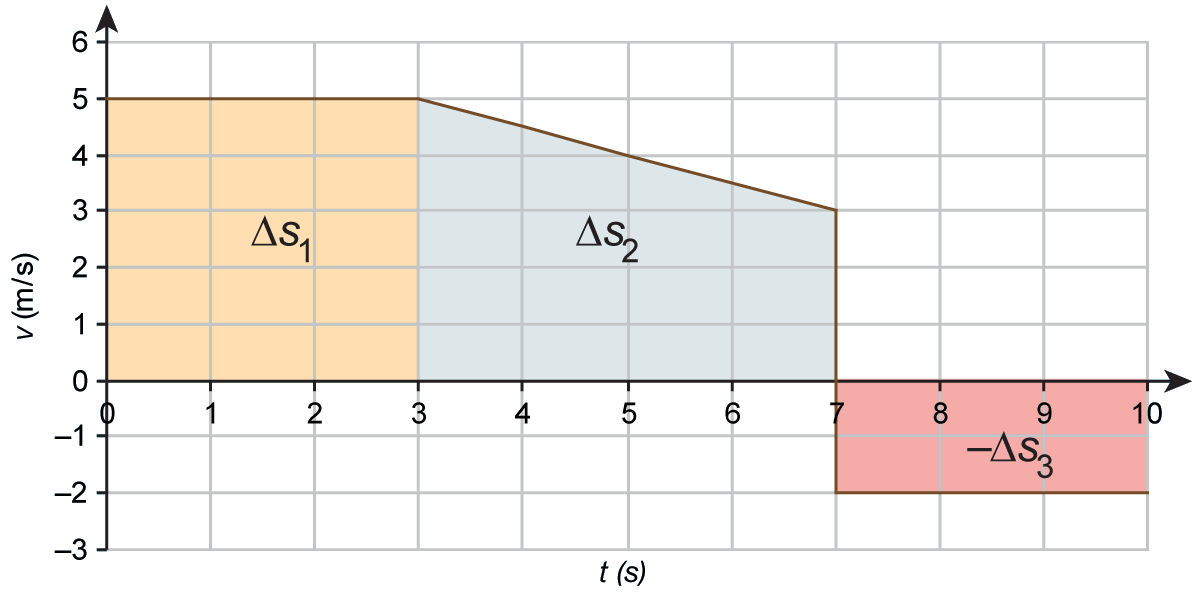
\includegraphics[width=\textwidth]{../images/chapter3/velocityTime.png}
\caption{Hastighet-tid diagram. Källa: Impuls Fysik 1}
\end{figure}
Accelerationen är lutningen på kurvan, sträckan är arean under grafen. Observera att negativ sträcka betyder att
föremålet rör sig tillbaka mot noll-punkten.
\begin{figure}[!h]
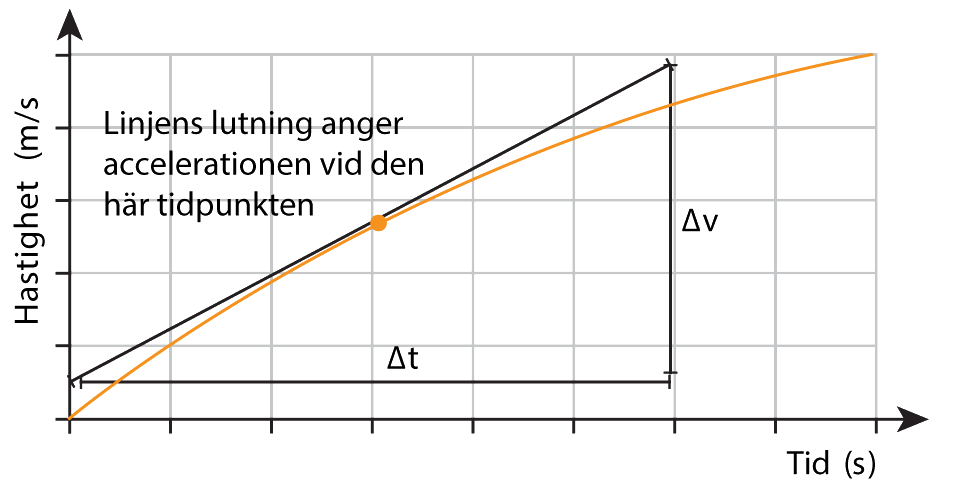
\includegraphics[width=0.5\textwidth]{../images/chapter3/velocityTimeAcceleration.png}
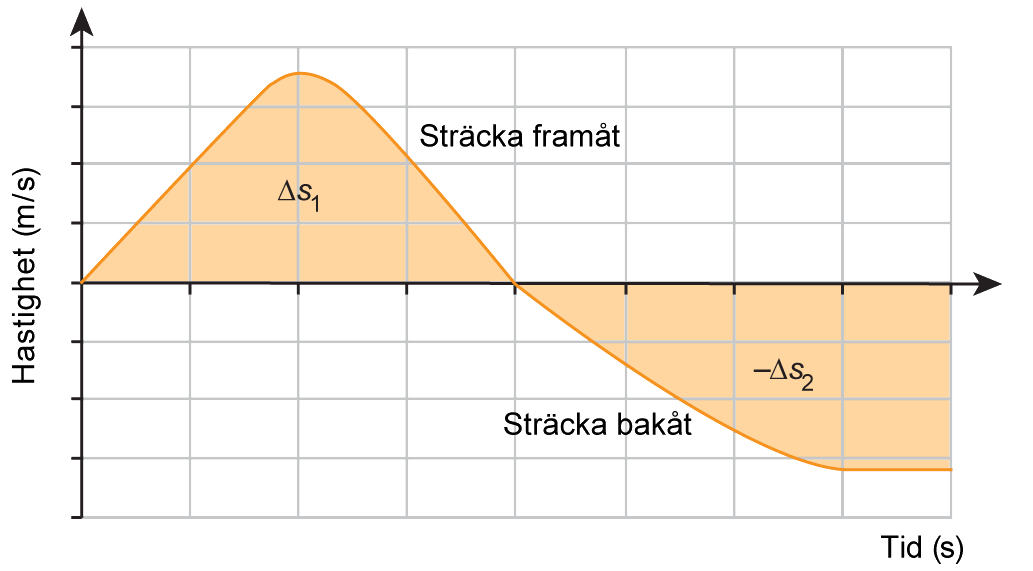
\includegraphics[width=0.5\textwidth]{../images/chapter3/velocityTimeDist.png}
\caption{Hastighet-tid diagram. Källa: Impuls Fysik 1}
\end{figure}
\clearpage
\section{Acceleration-tid-diagram}
\begin{figure}[!h]
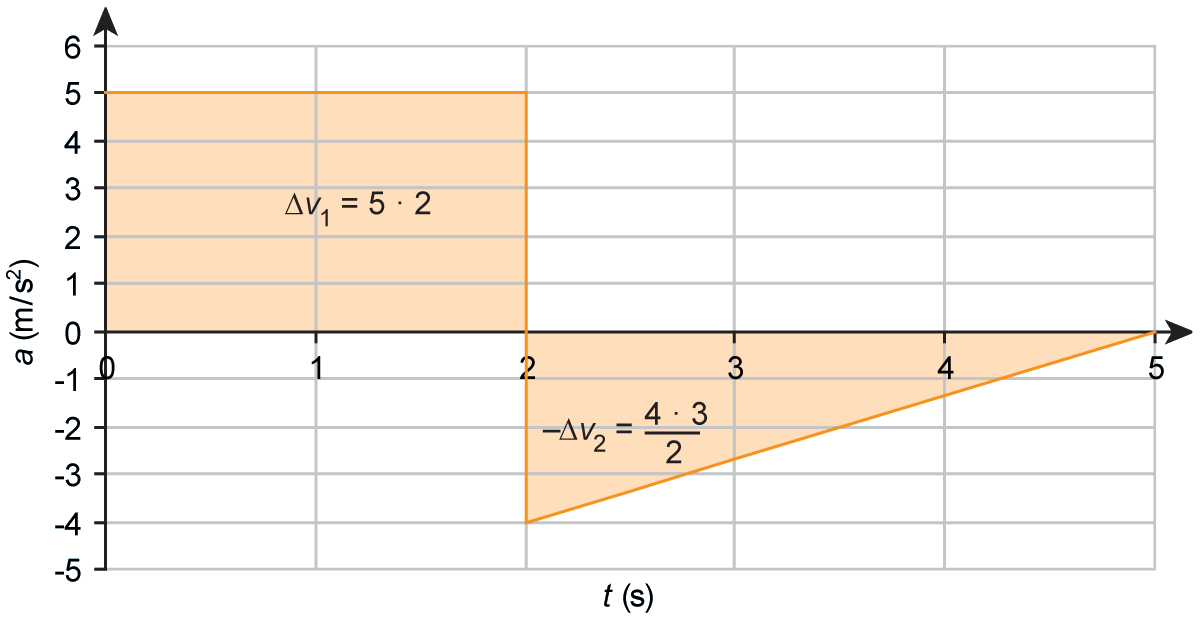
\includegraphics[width=\textwidth]{../images/chapter3/accelerationTime.png}
\caption{Acceleration-tid diagram. Källa: Impuls Fysik 1}
\end{figure}
Förändringen av hastighet är arean under grafen.
\clearpage
\section{Planering}
\begin{table}{|r|r|r|r}
    %! Author = magnus.silverdal
%! Date = 2020-09-24


\hline
17/9 && Momentanhastighet, medelhastighet och hastighet som vektor. && Sidorna 46-51 && uppgifterna 302-316, lös de jämna uppgifterna bara. \\

18/9 && Sträcka-tid diagram och hastigheten som kurvans lutning (derivata) && Sidorna 52-55. && uppgifterna 318-326 \\

23/9 && Acceleration. && Sidorna 56-60, &&  uppgifterna 327-338 \\

24/9 && Hastighet-tid och acceleration-tid-diagram. && Sidorna 61-72, && uppgifterna fram till 349 \\

25/9 && Rörelse med konstant acceleration. De två viktigaste modellerna v=v0 + a t och s = v0
t + a t^2 / 2.  && Sidorna 73-77. &&  Uppgifterna 350-359. \\

1/10 && Repetition. && && Uppgifterna 360-391 \\

2/10 && Kunskapstest. Kapitel 3. Vi lånar tid från programmeringslektionen för att ni inte ska hamna i tidsnöd. && && \\

\hline

\end{table}

\end{document}